\documentclass[]{book}
\usepackage{lmodern}
\usepackage{amssymb,amsmath}
\usepackage{ifxetex,ifluatex}
\usepackage{fixltx2e} % provides \textsubscript
\ifnum 0\ifxetex 1\fi\ifluatex 1\fi=0 % if pdftex
  \usepackage[T1]{fontenc}
  \usepackage[utf8]{inputenc}
\else % if luatex or xelatex
  \ifxetex
    \usepackage{mathspec}
  \else
    \usepackage{fontspec}
  \fi
  \defaultfontfeatures{Ligatures=TeX,Scale=MatchLowercase}
\fi
% use upquote if available, for straight quotes in verbatim environments
\IfFileExists{upquote.sty}{\usepackage{upquote}}{}
% use microtype if available
\IfFileExists{microtype.sty}{%
\usepackage{microtype}
\UseMicrotypeSet[protrusion]{basicmath} % disable protrusion for tt fonts
}{}
\usepackage[margin=1in]{geometry}
\usepackage{hyperref}
\hypersetup{unicode=true,
            pdftitle={Animal Environmental Science},
            pdfauthor={Sangrak Lee; Youngjun Na},
            pdfborder={0 0 0},
            breaklinks=true}
\urlstyle{same}  % don't use monospace font for urls
\usepackage{natbib}
\bibliographystyle{apalike}
\usepackage{longtable,booktabs}
\usepackage{graphicx,grffile}
\makeatletter
\def\maxwidth{\ifdim\Gin@nat@width>\linewidth\linewidth\else\Gin@nat@width\fi}
\def\maxheight{\ifdim\Gin@nat@height>\textheight\textheight\else\Gin@nat@height\fi}
\makeatother
% Scale images if necessary, so that they will not overflow the page
% margins by default, and it is still possible to overwrite the defaults
% using explicit options in \includegraphics[width, height, ...]{}
\setkeys{Gin}{width=\maxwidth,height=\maxheight,keepaspectratio}
\IfFileExists{parskip.sty}{%
\usepackage{parskip}
}{% else
\setlength{\parindent}{0pt}
\setlength{\parskip}{6pt plus 2pt minus 1pt}
}
\setlength{\emergencystretch}{3em}  % prevent overfull lines
\providecommand{\tightlist}{%
  \setlength{\itemsep}{0pt}\setlength{\parskip}{0pt}}
\setcounter{secnumdepth}{5}
% Redefines (sub)paragraphs to behave more like sections
\ifx\paragraph\undefined\else
\let\oldparagraph\paragraph
\renewcommand{\paragraph}[1]{\oldparagraph{#1}\mbox{}}
\fi
\ifx\subparagraph\undefined\else
\let\oldsubparagraph\subparagraph
\renewcommand{\subparagraph}[1]{\oldsubparagraph{#1}\mbox{}}
\fi

%%% Use protect on footnotes to avoid problems with footnotes in titles
\let\rmarkdownfootnote\footnote%
\def\footnote{\protect\rmarkdownfootnote}

%%% Change title format to be more compact
\usepackage{titling}

% Create subtitle command for use in maketitle
\newcommand{\subtitle}[1]{
  \posttitle{
    \begin{center}\large#1\end{center}
    }
}

\setlength{\droptitle}{-2em}

  \title{Animal Environmental Science}
    \pretitle{\vspace{\droptitle}\centering\huge}
  \posttitle{\par}
    \author{Sangrak Lee; Youngjun Na}
    \preauthor{\centering\large\emph}
  \postauthor{\par}
      \predate{\centering\large\emph}
  \postdate{\par}
    \date{Last update: 2019-02-20}

\usepackage{booktabs}

\begin{document}
\maketitle

{
\setcounter{tocdepth}{1}
\tableofcontents
}
\chapter*{Welcome}\label{welcome}
\addcontentsline{toc}{chapter}{Welcome}

This is the website for \textbf{``Animal environmental science''}. To
understanding individual animals, we have to understand the relationship
they have with their environment. This book will focus at the
interaction between animals and the environment.

This website is (and will always be) \textbf{free to use}, and is
licensed under the
\href{http://creativecommons.org/licenses/by-nc-nd/3.0/us/}{Creative
Commons Attribution-NonCommercial-NoDerivs 3.0} License. The book is
written in \href{https://rmarkdown.rstudio.com}{RMarkdown} with
\href{https://bookdown.org}{bookdown}. Some photographs used in this
book was from \href{https://unsplash.com/}{Unsplash.com}. If you click
the download button up above, you can download the PDF version of the
book.

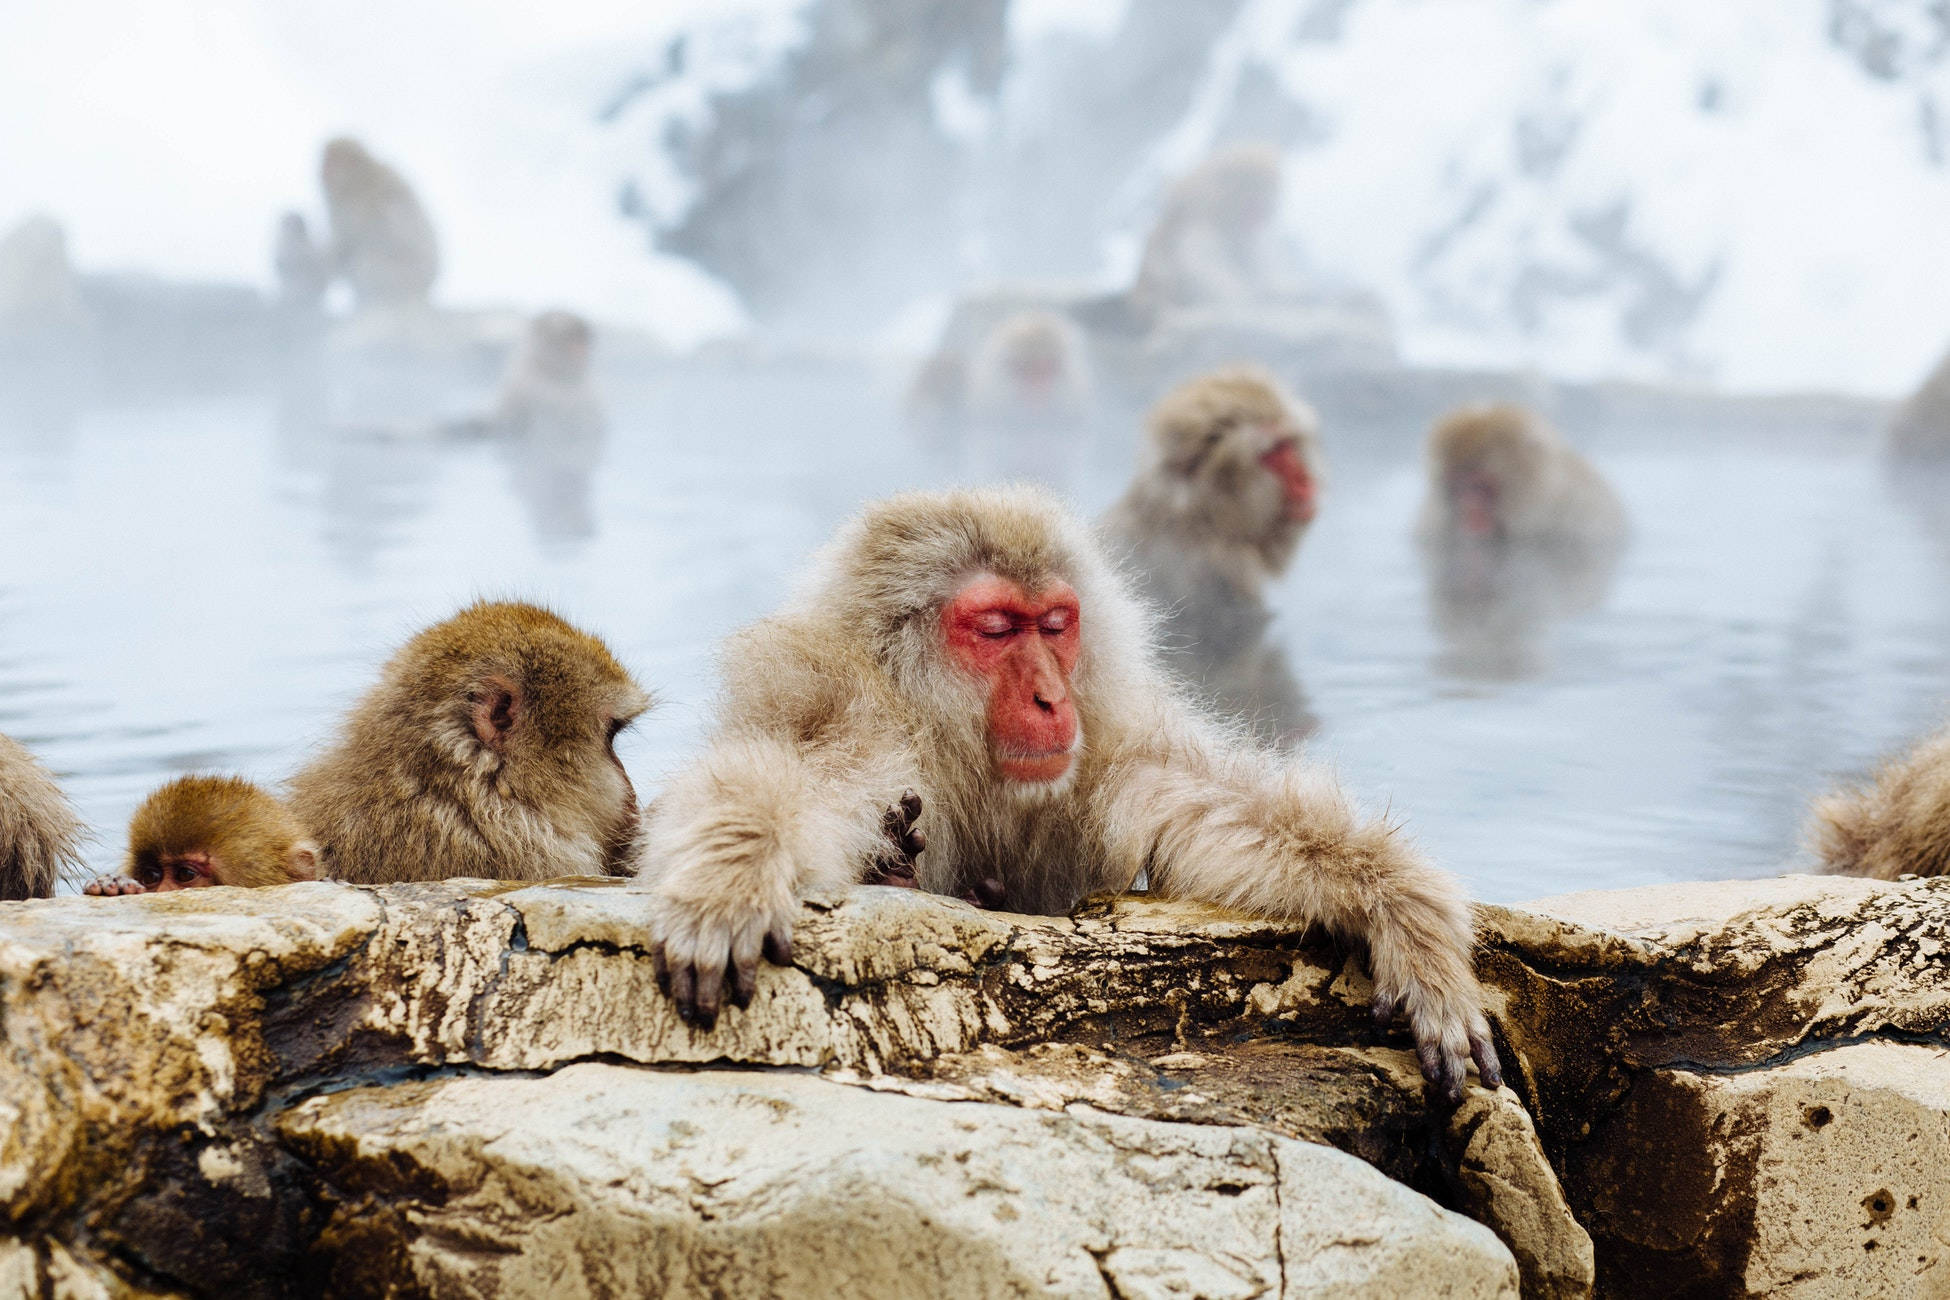
\includegraphics{figures/monkey.jpeg}\\
(Snow Monkey Niseko, Kutchan-chō, Japan)

\chapter{Introduction}\label{intro}

All living creatures constantly interact with the environment. To
understanding individual animals, we have to understand the relationship
they have with their environment. Also, animals affect the environment.
From birth to death, animals generate carbon dioxide, methane, feces,
and urine. The excretes from animals are builded with molecules such as
carbon, nitrogen, sulfur, and phosphorus, and are recycled within and
between ecosystems.

Basically, animals can find food, shelter, protection, and mates from
the environment called \emph{habitat}. The animal habitat includes both
phisical (non-living) and biotic (livinig) components (see Table
\ref{tab:habitat}).

\begin{table}[t]

\caption{\label{tab:habitat}Components of habitat (physical and biotic)}
\centering
\begin{tabular}{ll}
\toprule
Physical & Biotic\\
\midrule
Temperature & Plant matter\\
Humidity & Predators\\
Oxygen & Parasites\\
Wind & Competitors\\
Soil & Individuals of the same species\\
\addlinespace
Light intensity & \\
Elevation & \\
\bottomrule
\end{tabular}
\end{table}

Animal habitat is constantly changed over time. Not only natural
disasters (eruption of volcano, earthquake, tsunami, and wildfire), also
human activity can affect the animal habitat. Unlike the wildlife, the
environment of domesticated animals (such as cow, pig, poultry, and dog)
that raised in the facility are controlled by the human. Because it's a
very huge field, this book can't cover every topic of both wildlife and
domesticated animal. Thus, from now on, we will deal with the topic for
the domesticated animal.

\begin{figure}

{\centering 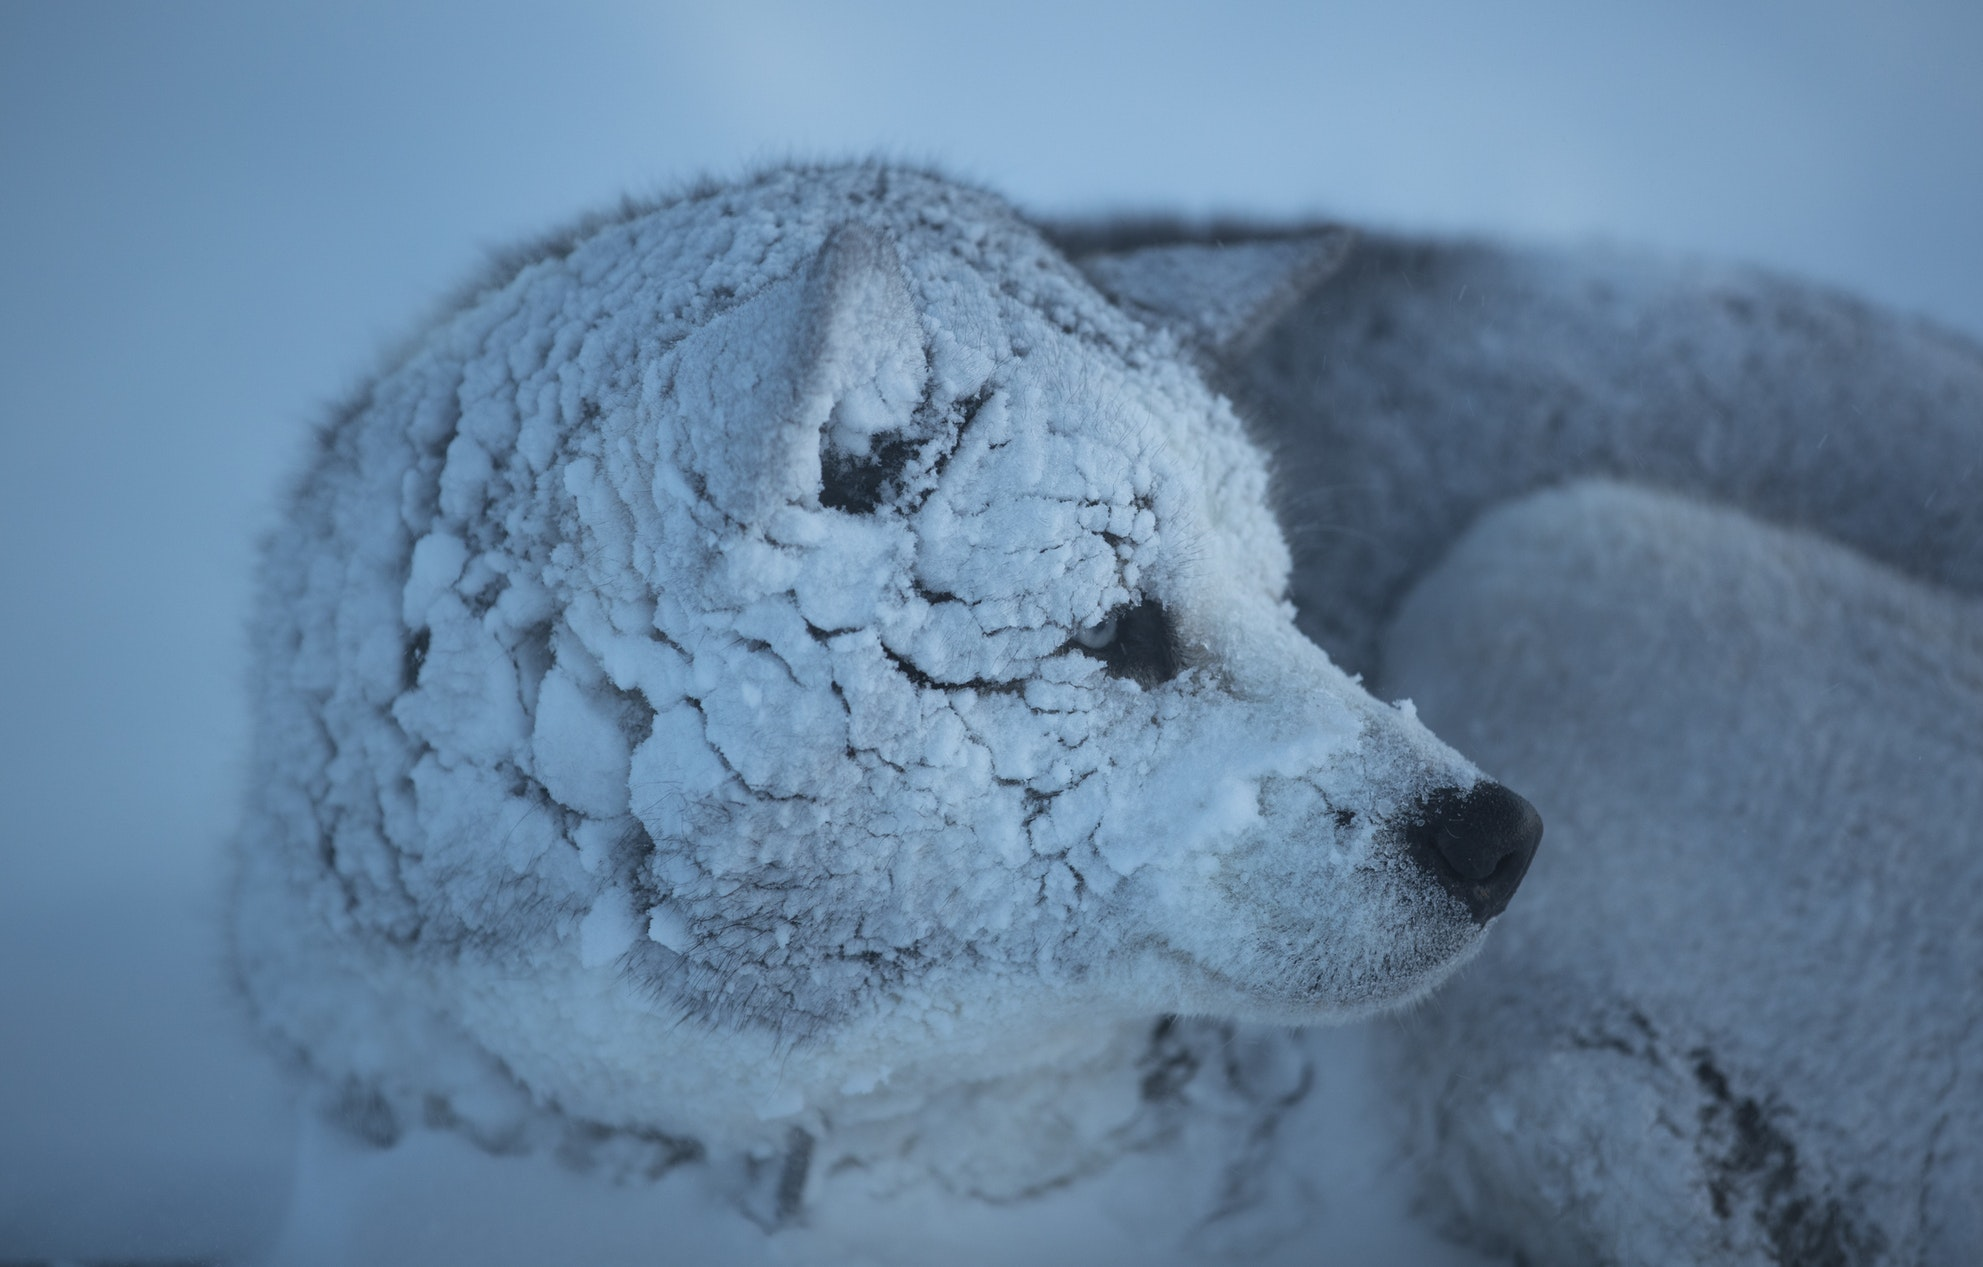
\includegraphics[width=0.6\linewidth]{figures/polar} 

}

\caption{Alaskan Malamute has the heat-conserving features.}\label{fig:snow-dog}
\end{figure}

\chapter{Animal and environment}\label{chapter2}

\section{External environment}\label{external-environment}

Animal never separates from the stimuli from outside. In the domestic
animals, the external environment includes both physical (e.g.~housing,
feeder, paddock, fence, and noise) and biotic (e.g.~human, mate, and
feed ingredients) components like those of animal habitat \ref{intro}.

\begin{figure}

{\centering 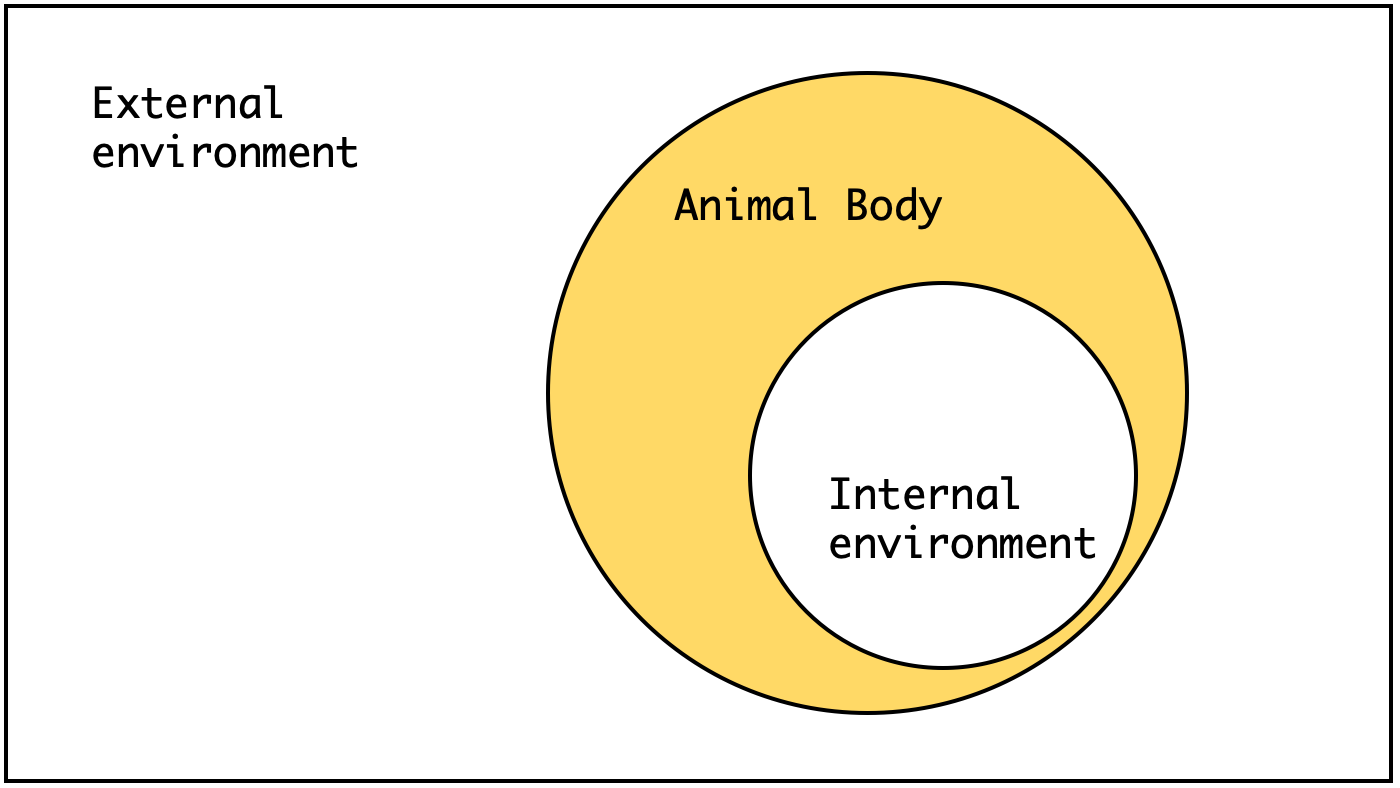
\includegraphics[width=0.6\linewidth]{figures/animal-env} 

}

\caption{External and internal environment}\label{fig:ext-int-env}
\end{figure}

\section{Internal environment}\label{internal-environment}

\begin{quote}
``The living body, though it has need of the surrounding environment, is
nevertheless relatively independent of it.'' --- Claude Bernard
\end{quote}

Higher animals have complex organ systems that respond to stimuli to
perform their essential body functions. When the animal receives the
signals from the sensory organs, they produce a local reflex action
and/or react in the central nervous system. Weak signals produce no
responses, but strong stimuli change the physiological or behavioral
status of the animal.

\subsection{Shelford's law of
tolerance}\label{shelfords-law-of-tolerance}

\begin{quote}
``Each and every species is able to exist and reproduce successfully
only within a definite range of environmental conditions.'' --- Ronald
Good
\end{quote}

Although external environments are continuously changed, if animals in
the normal status, they keep the composition of the extracellular fluid
(internal environment) constant to maintain their life. We call it
\emph{homeostasis}.

\begin{table}[t]

\caption{\label{tab:homeostasis}List of homeostatic control variables}
\centering
\begin{tabular}{l}
\toprule
Control variables\\
\midrule
Core temperature; Blood glucose; Iron levels; Copper regulation; Levels of blood gases;\\
Blood oxygen content; Arterial blood pressure; Calcium levels; Sodium concentration;\\
Potassium concentration; Fluid balance; Blood pH; Cerebrospinal fluid; Neurotransmission;\\
Neuroendocrine system; Gene regulation; and Energy balance\\
\bottomrule
\end{tabular}
\end{table}

However, the capacity to maintain the homeostasis is broken when the
animals let the harsh environments and differ by their species.
\textbf{Animals may be limited in their growth and their occurrence by
the minimum, maximum, and optimum condition} \citep{shelford} (Fig.
\ref{fig:law-of-tol}).

\begin{figure}
\centering
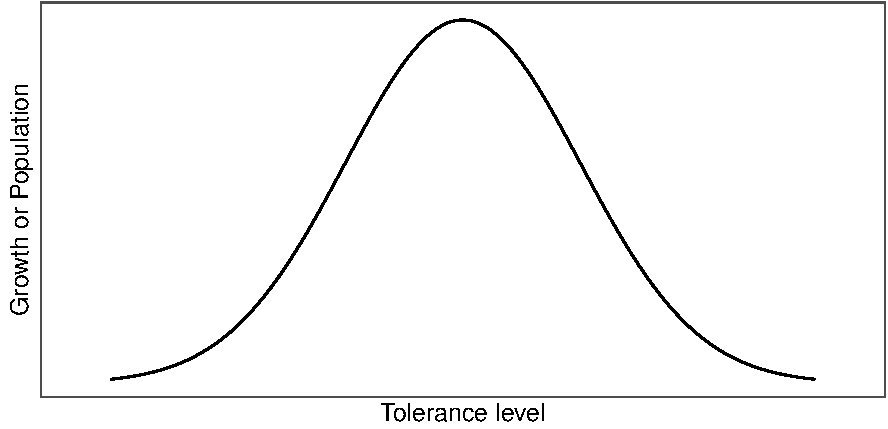
\includegraphics{AES_files/figure-latex/law-of-tol-1.pdf}
\caption{\label{fig:law-of-tol}Shelford's law of tolerance}
\end{figure}

The optimum range of environmental condition may differ within the same
organism, and it is not necessarily fixed. They can change as:

\begin{itemize}
\tightlist
\item
  Change of seasons
\item
  Change of environmental conditions
\item
  Life stage of the organism
\end{itemize}

\subsection{Adaptation}\label{adaptation}

\begin{quote}
``Changes in morphological, anatomical, physiological, biochemical and
behavioral characteristics of the animal which promote welfare and favor
survival in a specific environment.'' --- Hafez
\end{quote}

\citet{hafez1968adaptation} defined an adaptation as above. The
adaptation helps an animal survive in their external environment. The
representative adaptive traits are:

\begin{enumerate}
\def\labelenumi{\arabic{enumi}.}
\tightlist
\item
  Structural adaptation
\item
  Behavioral adaptation
\item
  Physiological adaptation
\end{enumerate}

Structural adaptation is the changes in physical features (e.g.~body
shape, skin, and internal organs) of the animal. Behavioral adaptation
is the changes in behaviors (e.g.~searching for food, mating,
vocalizations, and mitigation) of the animal. Physiological adaptation
is the changes in the animal body functions such as growth, temperature
regulation, and ionic balance. Sometimes, adapted animal create a new
species (\emph{speciation}).

\subsection{Acclimatization}\label{acclimatization}

Acclimatization is the physiological changes induced by a complex of
factors such as altitude, temperature, humidity, photoperiod, or pH.
Acclimatization is the short-term process (hours to weeks) by comparison
with adaptation (take place over many generations).

\chapter{Temperature}\label{temperature}

Temperature is a quantity expressing of the amount of heat. Because a
rate of every chemical reaction occurs in the animal's body is affected
by the temperature, it is a very important factor to all animals. Like
most chemical reactions, an enzyme-catalyzed reaction rate in the
animal's body increases as the temperature is raised. However, extremely
high or low temperature results in loss of activity or lose the
structure for most enzymes (\emph{denaturation}; Figure \ref{fig:q10}).

\begin{figure}

{\centering 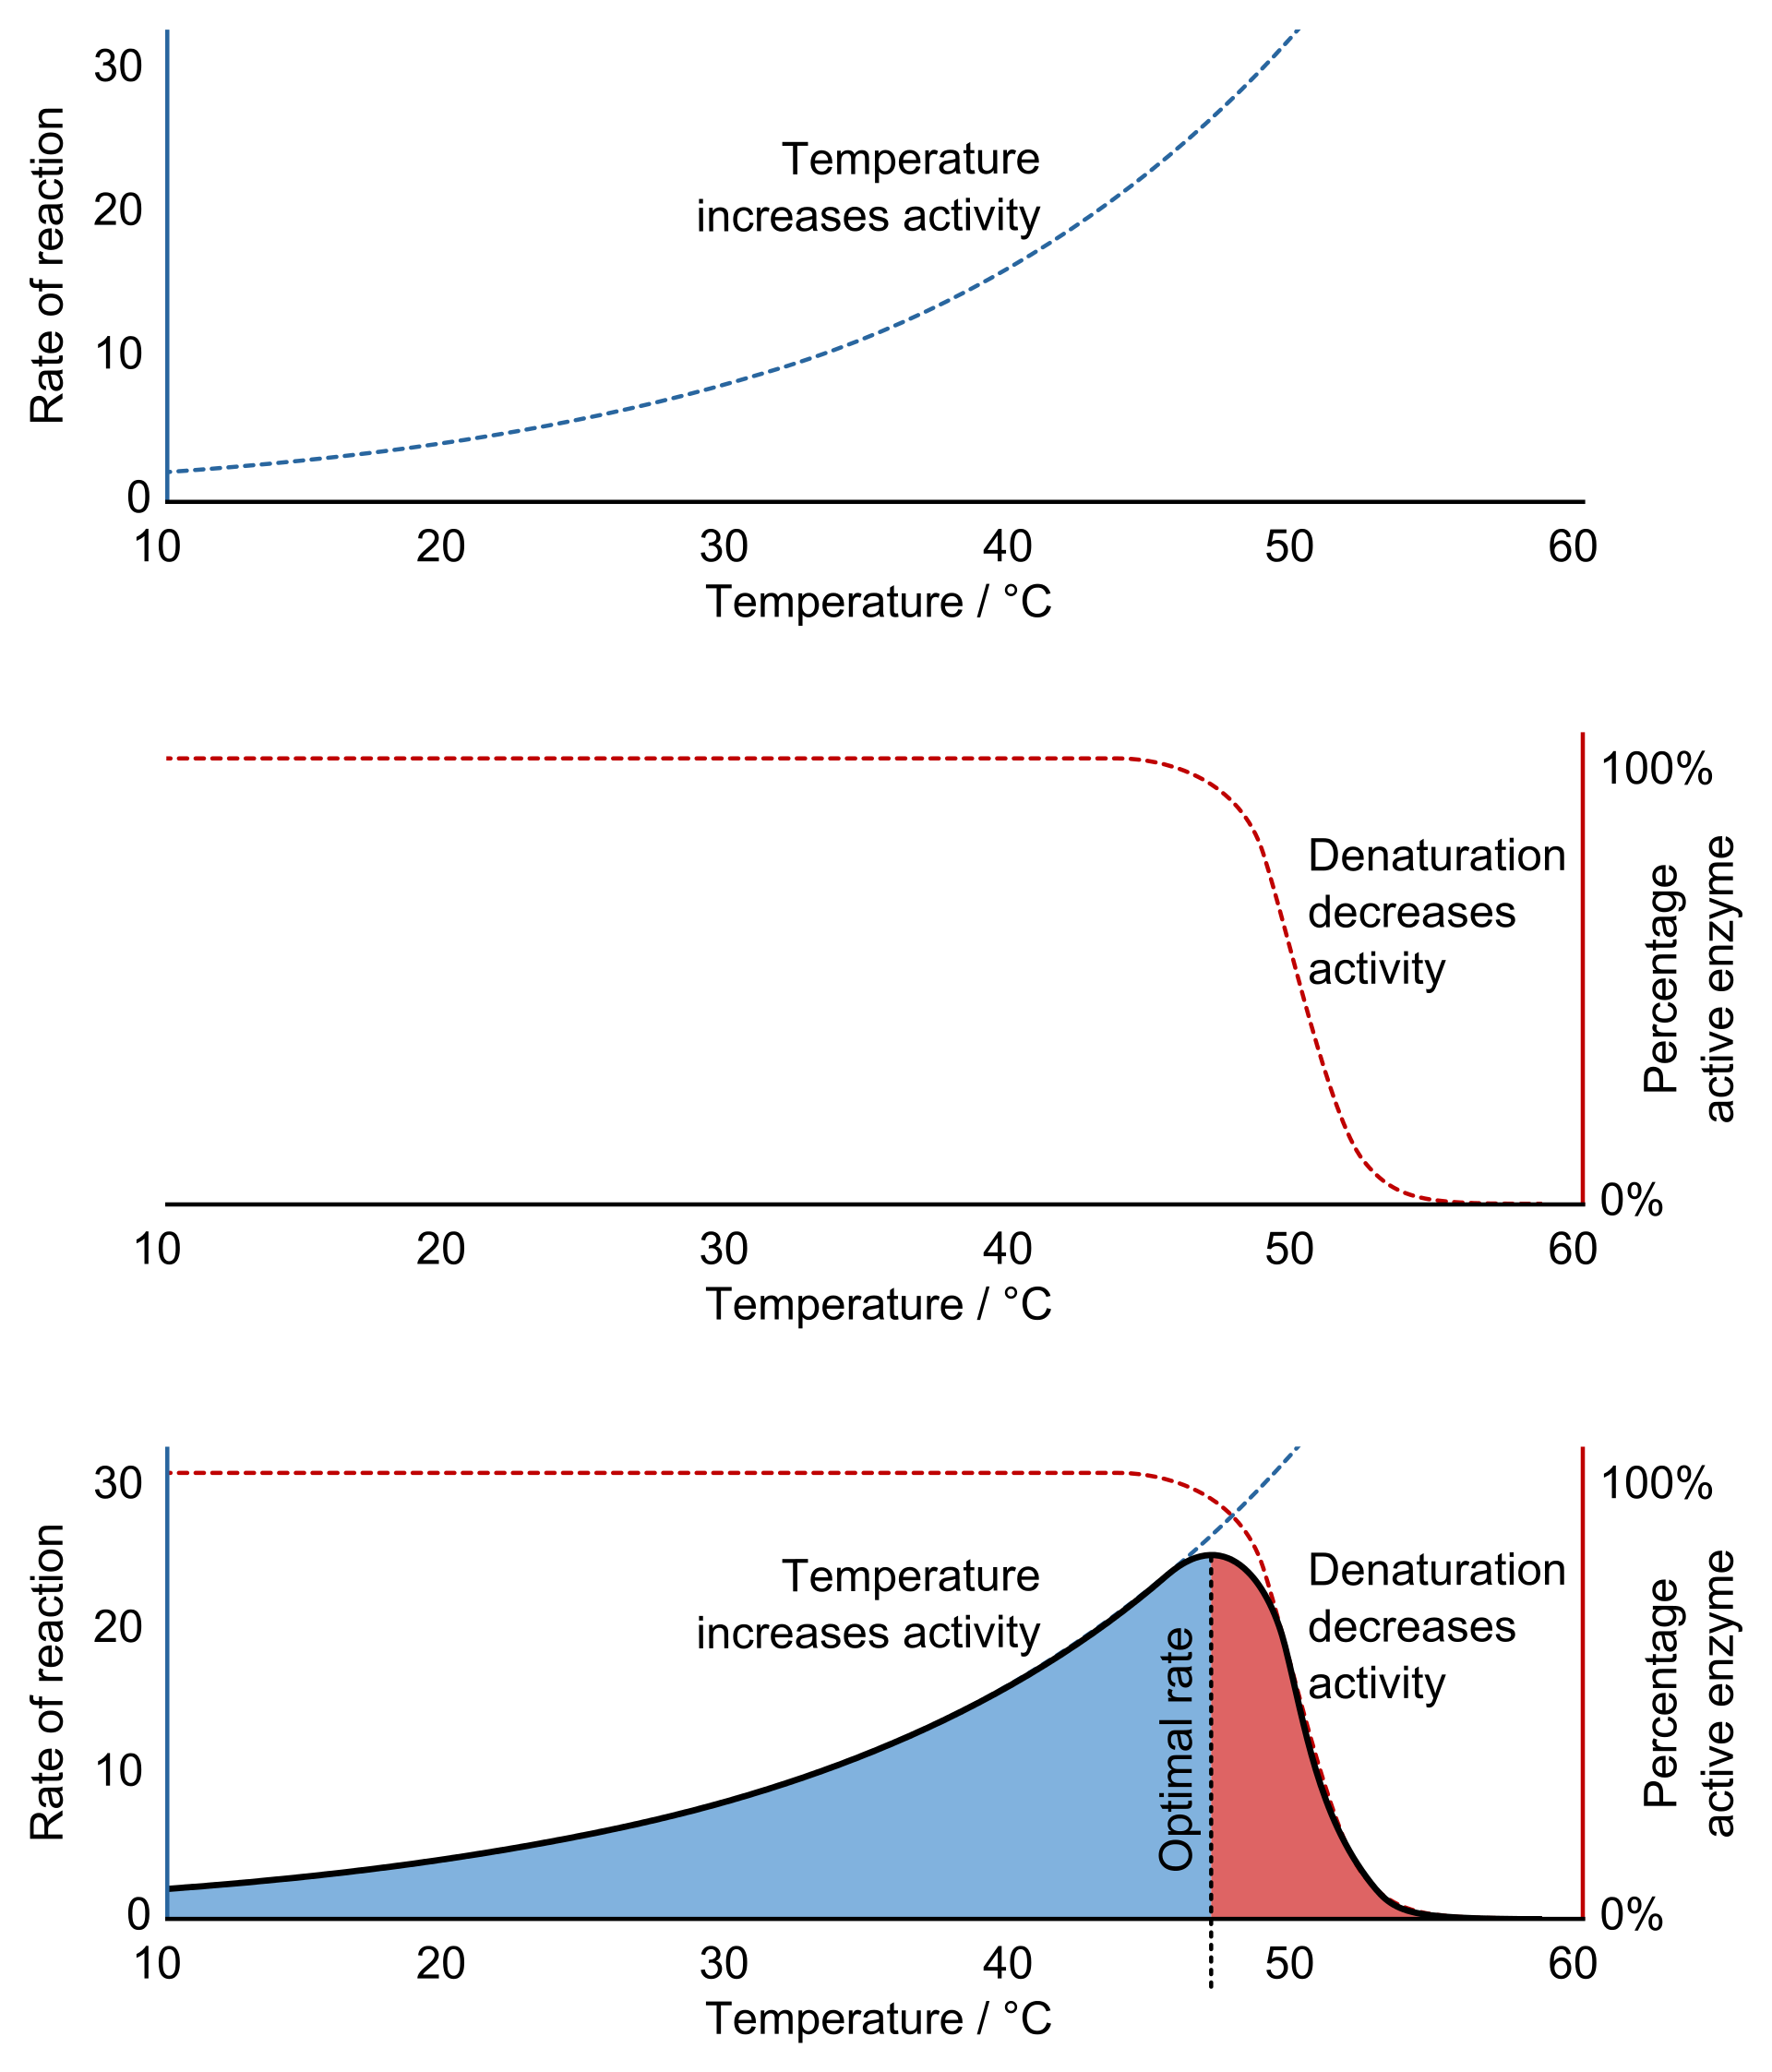
\includegraphics[width=0.6\linewidth]{figures/q10} 

}

\caption{The effects of temperature on enzyme activity [@q10]. Top - increasing temperature increases the rate of reaction (Q10 coefficient). Middle - the fraction of folded and functional enzyme decreases above its denaturation temperature. Bottom - consequently, an enzyme's optimal rate of reaction is at an intermediate temperature.}\label{fig:q10}
\end{figure}

\section{Poikilotherm and homeotherm}\label{poikilotherm-and-homeotherm}

Key factors for animal surviving are to adapt to external environmental
changes and maintain a consistent internal environment. The animal can
be divided into two types for response to external temperatures:
\emph{poikilotherm} (cold-blooded animals) and \emph{homeotherm}
(warm-blooded animals). Examples of poikilotherms are most fish,
amphibians, and reptiles. Their internal body temperature varies
considerably according to their external environments. On the other
hand, homeotherm maintains their thermal homeostasis. The examples of
homeotherm are birds and mammals.

\begin{figure}

{\centering 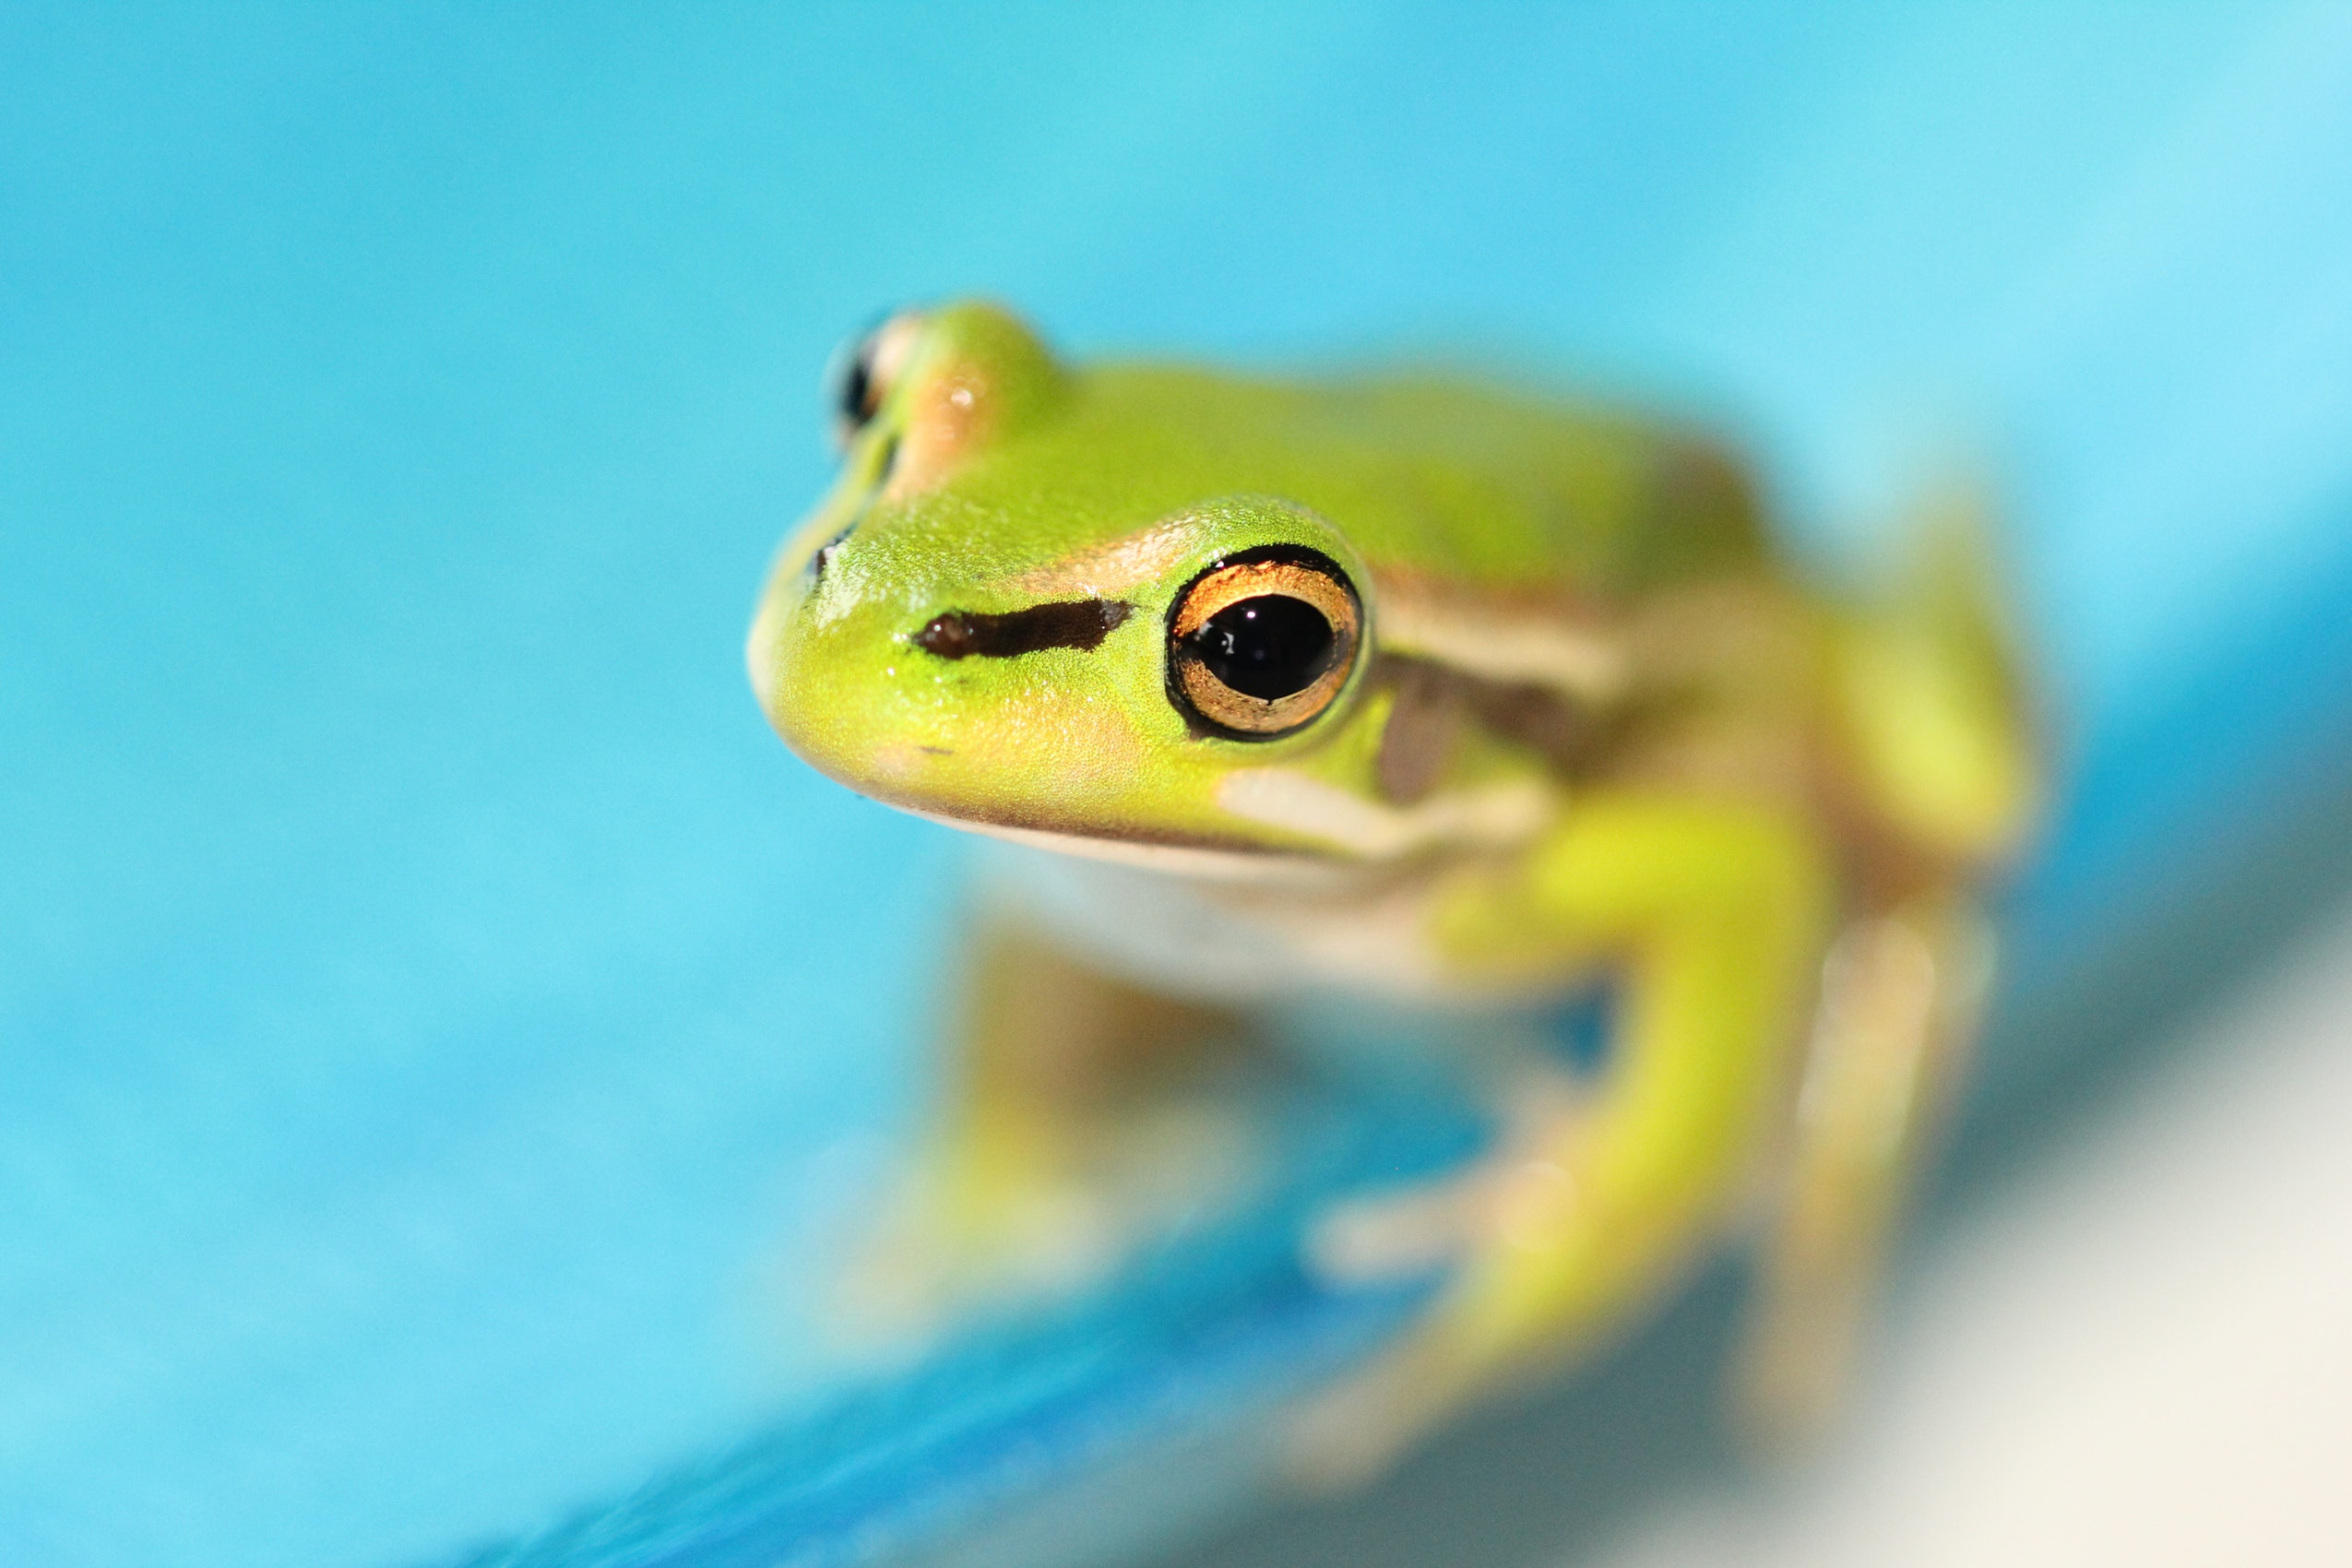
\includegraphics[width=1\linewidth]{figures/flog} 

}

\caption{Green frog on blue surface.}\label{fig:flor}
\end{figure}

\section{Thermoregulation}\label{thermoregulation}

\begin{table}[t]

\caption{\label{tab:norm-body-temp}Normal body temperature of the domestic animals; Body temperatures may be 1°C above or below these temperatures.}
\centering
\begin{tabular}{llll}
\toprule
Animal & Normal temperature (°C) & Animal & Normal temerature (°C)\\
\midrule
Cattle & 38.5 & Donkey & 38.2\\
Calf & 39.5 & Chicken & 42.0\\
Buffalo & 38.2 & Camel & 34.5-41.0\\
Sheep & 39.0 & Horse & 38.0\\
Llama, alpaca & 38.0 & Pig & 39.0\\
\addlinespace
Goat & 39.5 & Piglet & 39.8\\
\bottomrule
\end{tabular}
\end{table}

\section{Temperature humadity index
(THI)}\label{temperature-humadity-index-thi}

The productivity of domestic animals is primarily affected by air
temperature, and altered by wind, humidity, and radiation.

\section{Effects on production}\label{effects-on-production}

\subsection{Dairy cattle}\label{dairy-cattle}

\subsection{Beef cattle}\label{beef-cattle}

\subsection{Swine}\label{swine}

\subsection{Poultry}\label{poultry}

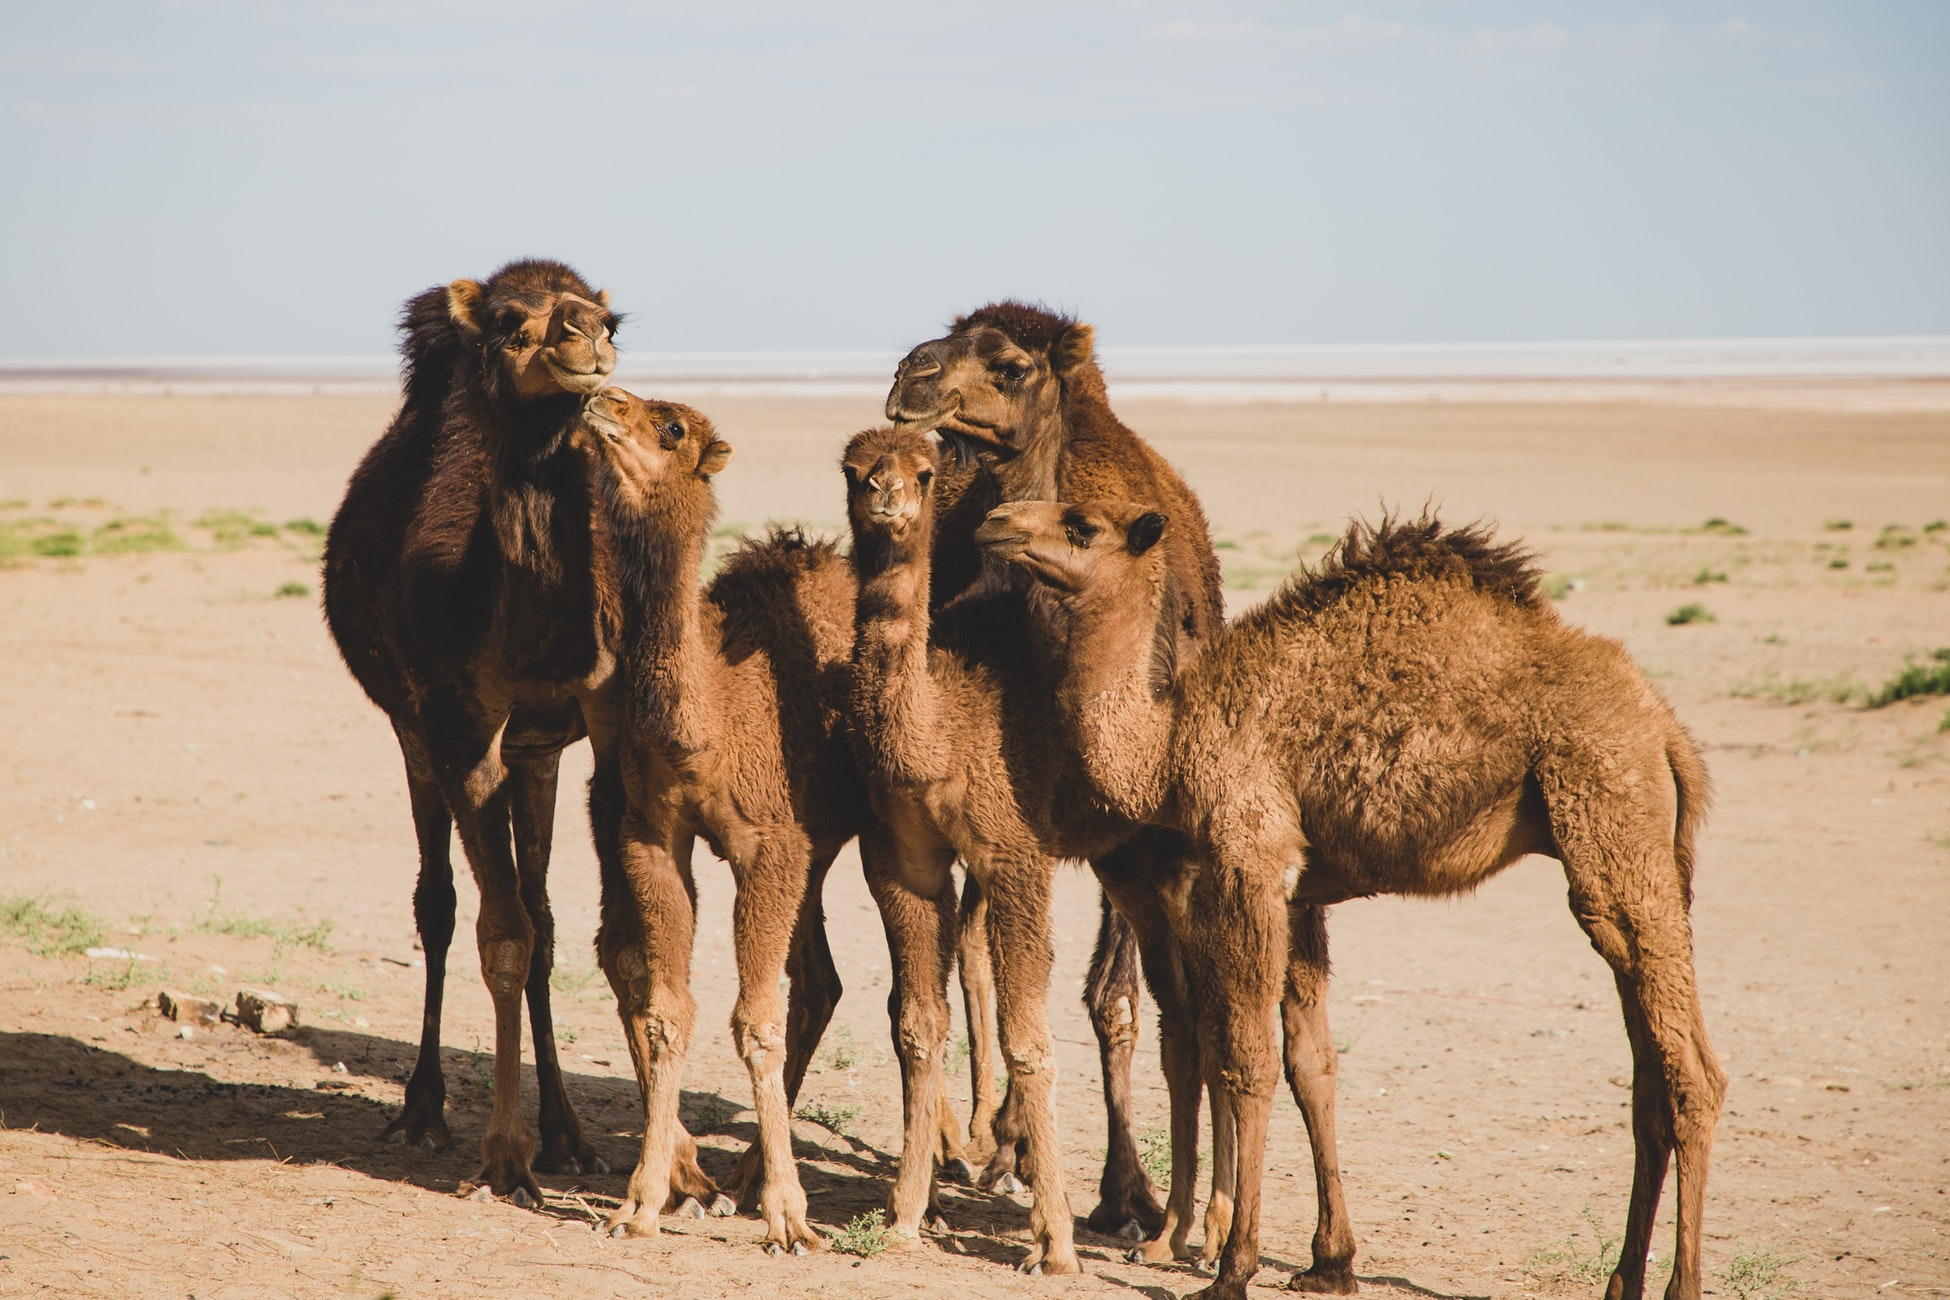
\includegraphics{figures/camels.jpeg} (Isfahan Province, Aran o Bidgol,
Iran)

\chapter{Light}\label{light}

\section{Photoperiodic response}\label{photoperiodic-response}

\section{Effects on productivity}\label{effects-on-productivity}

\subsection{Wool}\label{wool}

\subsection{Feathers}\label{feathers}

\subsection{Antlers}\label{antlers}

\subsection{Puberty}\label{puberty}

\subsection{Reproduction}\label{reproduction}

\subsection{Behavior}\label{behavior}

\subsection{Light control in poultry
production}\label{light-control-in-poultry-production}

\chapter{Sound}\label{sound}

\chapter{Air quality}\label{air-quality}

\chapter{Water quality}\label{water-quality}

\chapter{Cycles of materials}\label{cycles-of-materials}

\section{Ecosystem}\label{ecosystem}

\section{Trophic level}\label{trophic-level}

\section{Carbon cycle}\label{carbon-cycle}

\section{Nitrogen cycle}\label{nitrogen-cycle}

\section{Calcium and Phosphorus
cycle}\label{calcium-and-phosphorus-cycle}

\chapter{Manure}\label{manure}

\section{Charateristics of animal
manure}\label{charateristics-of-animal-manure}

\section{Manure treatment}\label{manure-treatment}

\subsection{Composting}\label{composting}

\subsection{Liquid fertilizer}\label{liquid-fertilizer}

\subsection{Purification}\label{purification}

\subsection{Energy generation}\label{energy-generation}

\subsection{Animal feed}\label{animal-feed}

\chapter{Greenhouse gases}\label{greenhouse-gases}

Here is a review of existing methods.

\chapter{Animal welfare}\label{animal-welfare}

Here is a review of existing methods.

\chapter{Sustainable livestock
industry}\label{sustainable-livestock-industry}

\begin{quote}
``In essence, the conflict between livestock and the environment is a
conflict between different human needs and expectations.'' --- Henning
Steinfeld (FAO)
\end{quote}

\bibliography{book.bib,packages.bib}


\end{document}
